% !Mode:: "TeX:UTF-8"
\chapter{bullet引擎的web移植}

\section{bullet引擎简介}

游戏引擎的概念诞生于上个世纪90年代的中期,与id Software公司的游戏《毁灭战士(Doom)》开发源码之家相关。《毁灭战士》的软件源码中,将游戏的软件架构划分成了游戏核心软件组件 (包括音频系统,碰撞检测系统,三维图形渲染系统等)、美术资源、游戏世界、构成玩家游戏体验的游戏规则几个部分。之后游戏引擎继续发展,简化为了资产管理、渲染循环、逻辑控制三个主要部分。

有了游戏引擎,游戏行业的从业者可以把注意力放在游戏的设计和逻辑实现上。不用因为游戏面向平台的系统架构、运行时内存管理、游戏画面的渲染绘制过程、物理碰撞检测实现等一些底层技术消耗太多精力。三维物理引擎是三维游戏引擎核心软件部分的重要组成部分。他的原理是在一个虚拟的空间中计算物体的相当位置,已经典的牛顿力学作为依据,计算在某个特定的时刻某个物体在物理空间中的特定坐标,然后将此坐标传递给渲染空间中的物体,并最后显示给用户,让用户体验到逼真的物理效果。

Bullet Physics Engine是一个开源的三维物理模拟引擎,世界三大三维物理引擎之一(另外两个是Intel的Havok,已经卖给微软和和Nvidia的PhysX)。广泛应用于游戏开发 (如EA的《模拟城市》,Rockstar的《GTA4》) 和电影 (如《2012》,《闪电狗》) 制作中,是AMD开放物理计划(Open Physics)核心成员之一\upcite{joselli2008new}。

绝大部分物理引擎(比如《游戏物理引擎开发》)的教材,可能都会把ODE\upcite{smith2013open} (Open Dynamics Engine) 当做主要教授的内容。但是,实际上,开源物理引擎的霸主是Bullet Physics。(但是最近,Nvidia也把Phsyx引擎开源了,所以霸主应该异位到了PhsyX)。Bullet Physics 是专业高效可靠的开源物理引擎,在AMD的开放物理计划的助力下,bullet引擎吸纳了Pixelux的DMM引擎同时整合了AMD贡献的CPU+GPU混合加速模块和光滑粒子流体动力学 (SPH) 系统,可免费用于商业和非商业游戏的开发和影视制作。Bullet Physics由百分之90的C++和接近百分之8的C语言以及Lua代码写成,是一个跨几乎所有有三维渲染能力平台的物理模拟计算引擎。支持Windows、Linux、MAC、Playstation3、Playstation4、XBOX360、XBOX ONE、Nintendo Wii、Nintendo 3DS。Bullet也整合到了动画建模软件Maya和Blender 3D(Blender game engine)当中。

\section{bullet引擎的程序的特征}

Bullet物理引擎和box2d一样,是一个需要把内部方法暴露出来,用来给别的语言调用的“白盒程序”,
或者叫框架或者类库。

在这种需求下,bullet引擎的移植同样需要使用webIDL技术。

bullet物理引擎也是模块开发的引擎,有如下模块:

\begin{itemize}[itemindent=2em]
    \item Bullet2FileLoader;
    \item Bullet3Collision;
    \item Bullet3Common;
    \item Bullet3Dynamics;
    \item Bullet3Geometry;
    \item Bullet3OpenCL;
    \item BulletCollision;
    \item BulletDynamics;
    \item BulletSoftBody;
    \item LinearMath。
\end{itemize}

在编译box2d时,为了方便,需要把所以box2d相关的组件,一次性编译到一个JavaScript文件中,对外是一个闭包的形式。但是bullet引擎不行。

Bullet引擎中,Bullet3标注的模块,是Bullet Physics加入AMD开发物理计划之后添加的,主要是支持openCL,支持GPU加速的物理模拟。
虽然,W3C和科诺斯已经完成了webCL标准的制定,但是现阶段没有一个原生支持webCL的浏览器。(诺基亚开发了firefox的webCL插件,三星开发了一个支持webCL版本的webkit)。总结一下,就是Bullet3相关的模块不能移植。而现代JavaScript虚拟机或者说现代浏览器为了安全,JavaScript代码在运行时采用了沙箱机制,禁止访问本机的文件,跨域访问文件和代码也做了非常明确的限制。因为Bullet2FileLoader也不应该也不能够进行移植。

所以,这次总共移植Bullet物理引擎的四个模块,这四个模块以及各自作用如下所示:

\begin{itemize}[itemindent=2em]
    \item BulletCollision,Bullet引擎的碰撞模块;
    \item BulletDynamics,Bullet引擎的动力学模块;
    \item BulletSoftBody,Bullet引擎的柔体模块;
    \item LinearMath,一个线性代数库。
\end{itemize}


\section{bullet引擎的程序的移植过程}

\subsection{bullet引擎的程序的移植过程}

编写bullet引擎的idl文件,具体可见附录中代码\ref{idl-bullet}所示。

Bullet物理引擎使用了cmake工具\upcite{martin2010mastering}完成构建。
emscripten也提供了工具emcmake,用来解析CmakeLists.txt文件。

而且,这次只编译其中一部分模块,还要手工打成一个闭包,以前使用make工具就显得不是很方便了。
我写了一个python脚本,具体为代码\ref{python-bullet-make-script},用来控制编译的过程。



之后,运行\ref{bash-bullet-build}所示的命令,可以得到builds/temp.js文件,也就是所要得到的bullet引擎移植到JavaScript的结果。

\begin{lstlisting}[
    language={bash},
    caption={bullet编译命令},
    label={bash-bullet-build},
]

# 在Bullet源码文件夹下运行,可以得到所有中间文件
./autogen.sh

# 在make.py所在文件夹下运行
python make.py
\end{lstlisting}



\subsection{bullet引擎的程序的移植过程分析}

bullet引擎的程序的移植过程分析如下:

\begin{enumerate}
    \item autogen.sh文件,先完成bullet引擎的编译;
    \item 使用idl文件(其中只包含BulletCollision、BulletDynamics、BulletSoftBody和LinearMath 4个模块的接口定义)生成胶水文件;
    \item 把编译后的四个模块文件(.a文件)反编译成字节码文件(.bc文件);
    \item 把字节码和胶水文件(glue.cpp,glue.js)一起编译成js文件;
	  \item 优化js文件。
\end{enumerate}

\subsection{bullet引擎在浏览器中的运行效果}

图\ref{ammo-sample-html}和图\ref{ammo-cloth}展示了bullet引擎在浏览器中运行的效果。第一个Demo展示了Bullet引擎计算碰撞的结果,并把坐标传递到三维空间各个物体的x、y和z三个坐标值上。第二个Demo则展示了Bullet引擎使用Softbody模块进行布料模拟的效果。

\newpage

\begin{figure}[h!] % [h!] 表示尽量排在当前位置
    \centering
    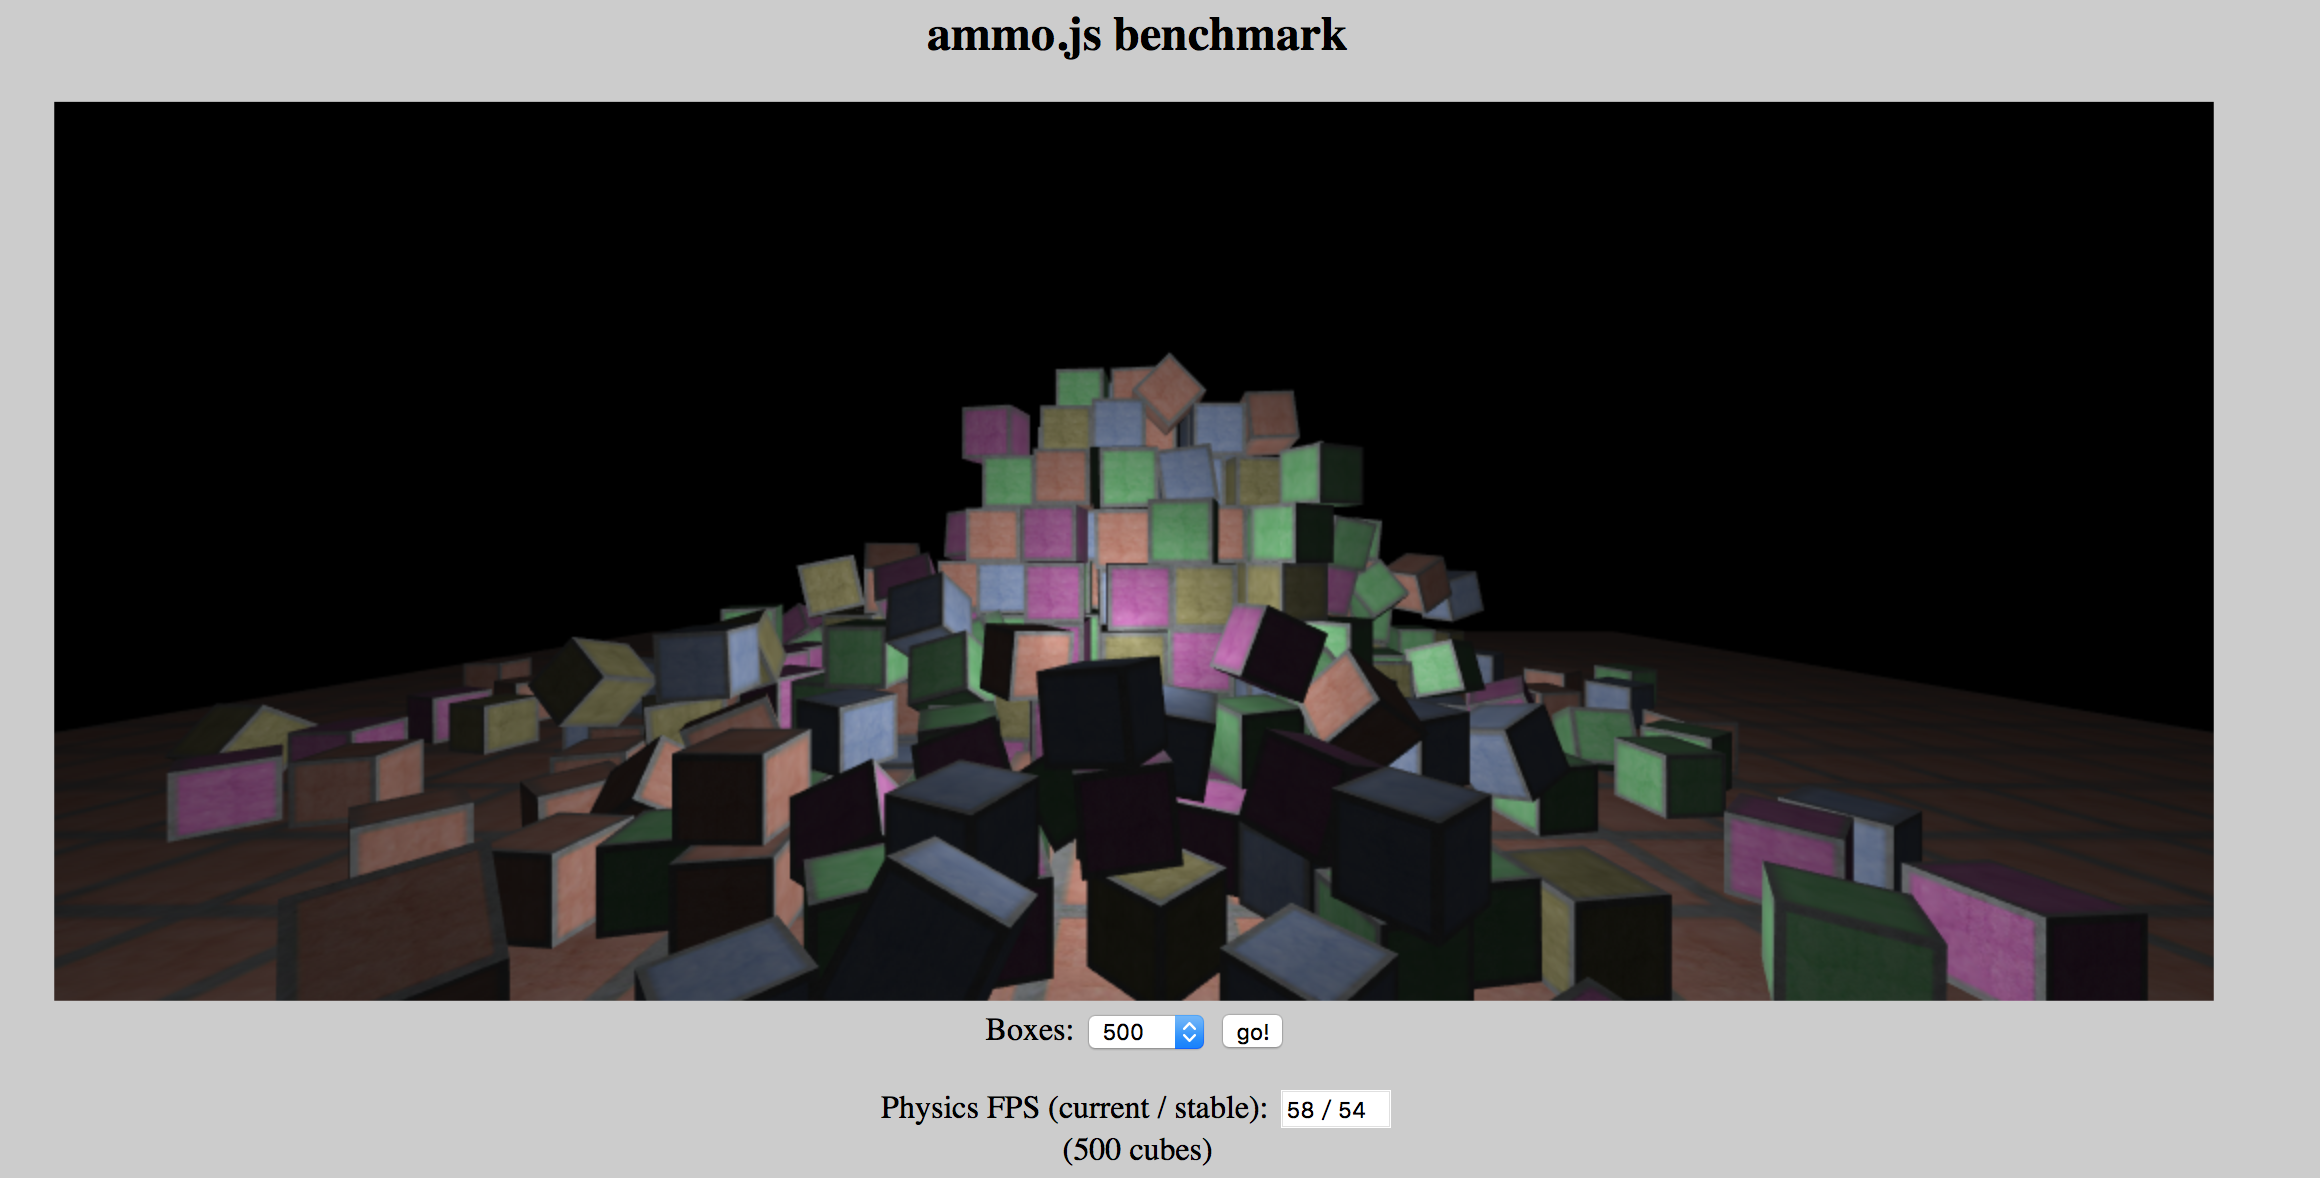
\includegraphics[width=450bp]{figure/pic/ammo-sample-html.png}
    \caption{bullet引擎在浏览器中运行效果}
    \label{ammo-sample-html}
\end{figure}

\begin{figure}[h!] % [h!] 表示尽量排在当前位置
    \centering
    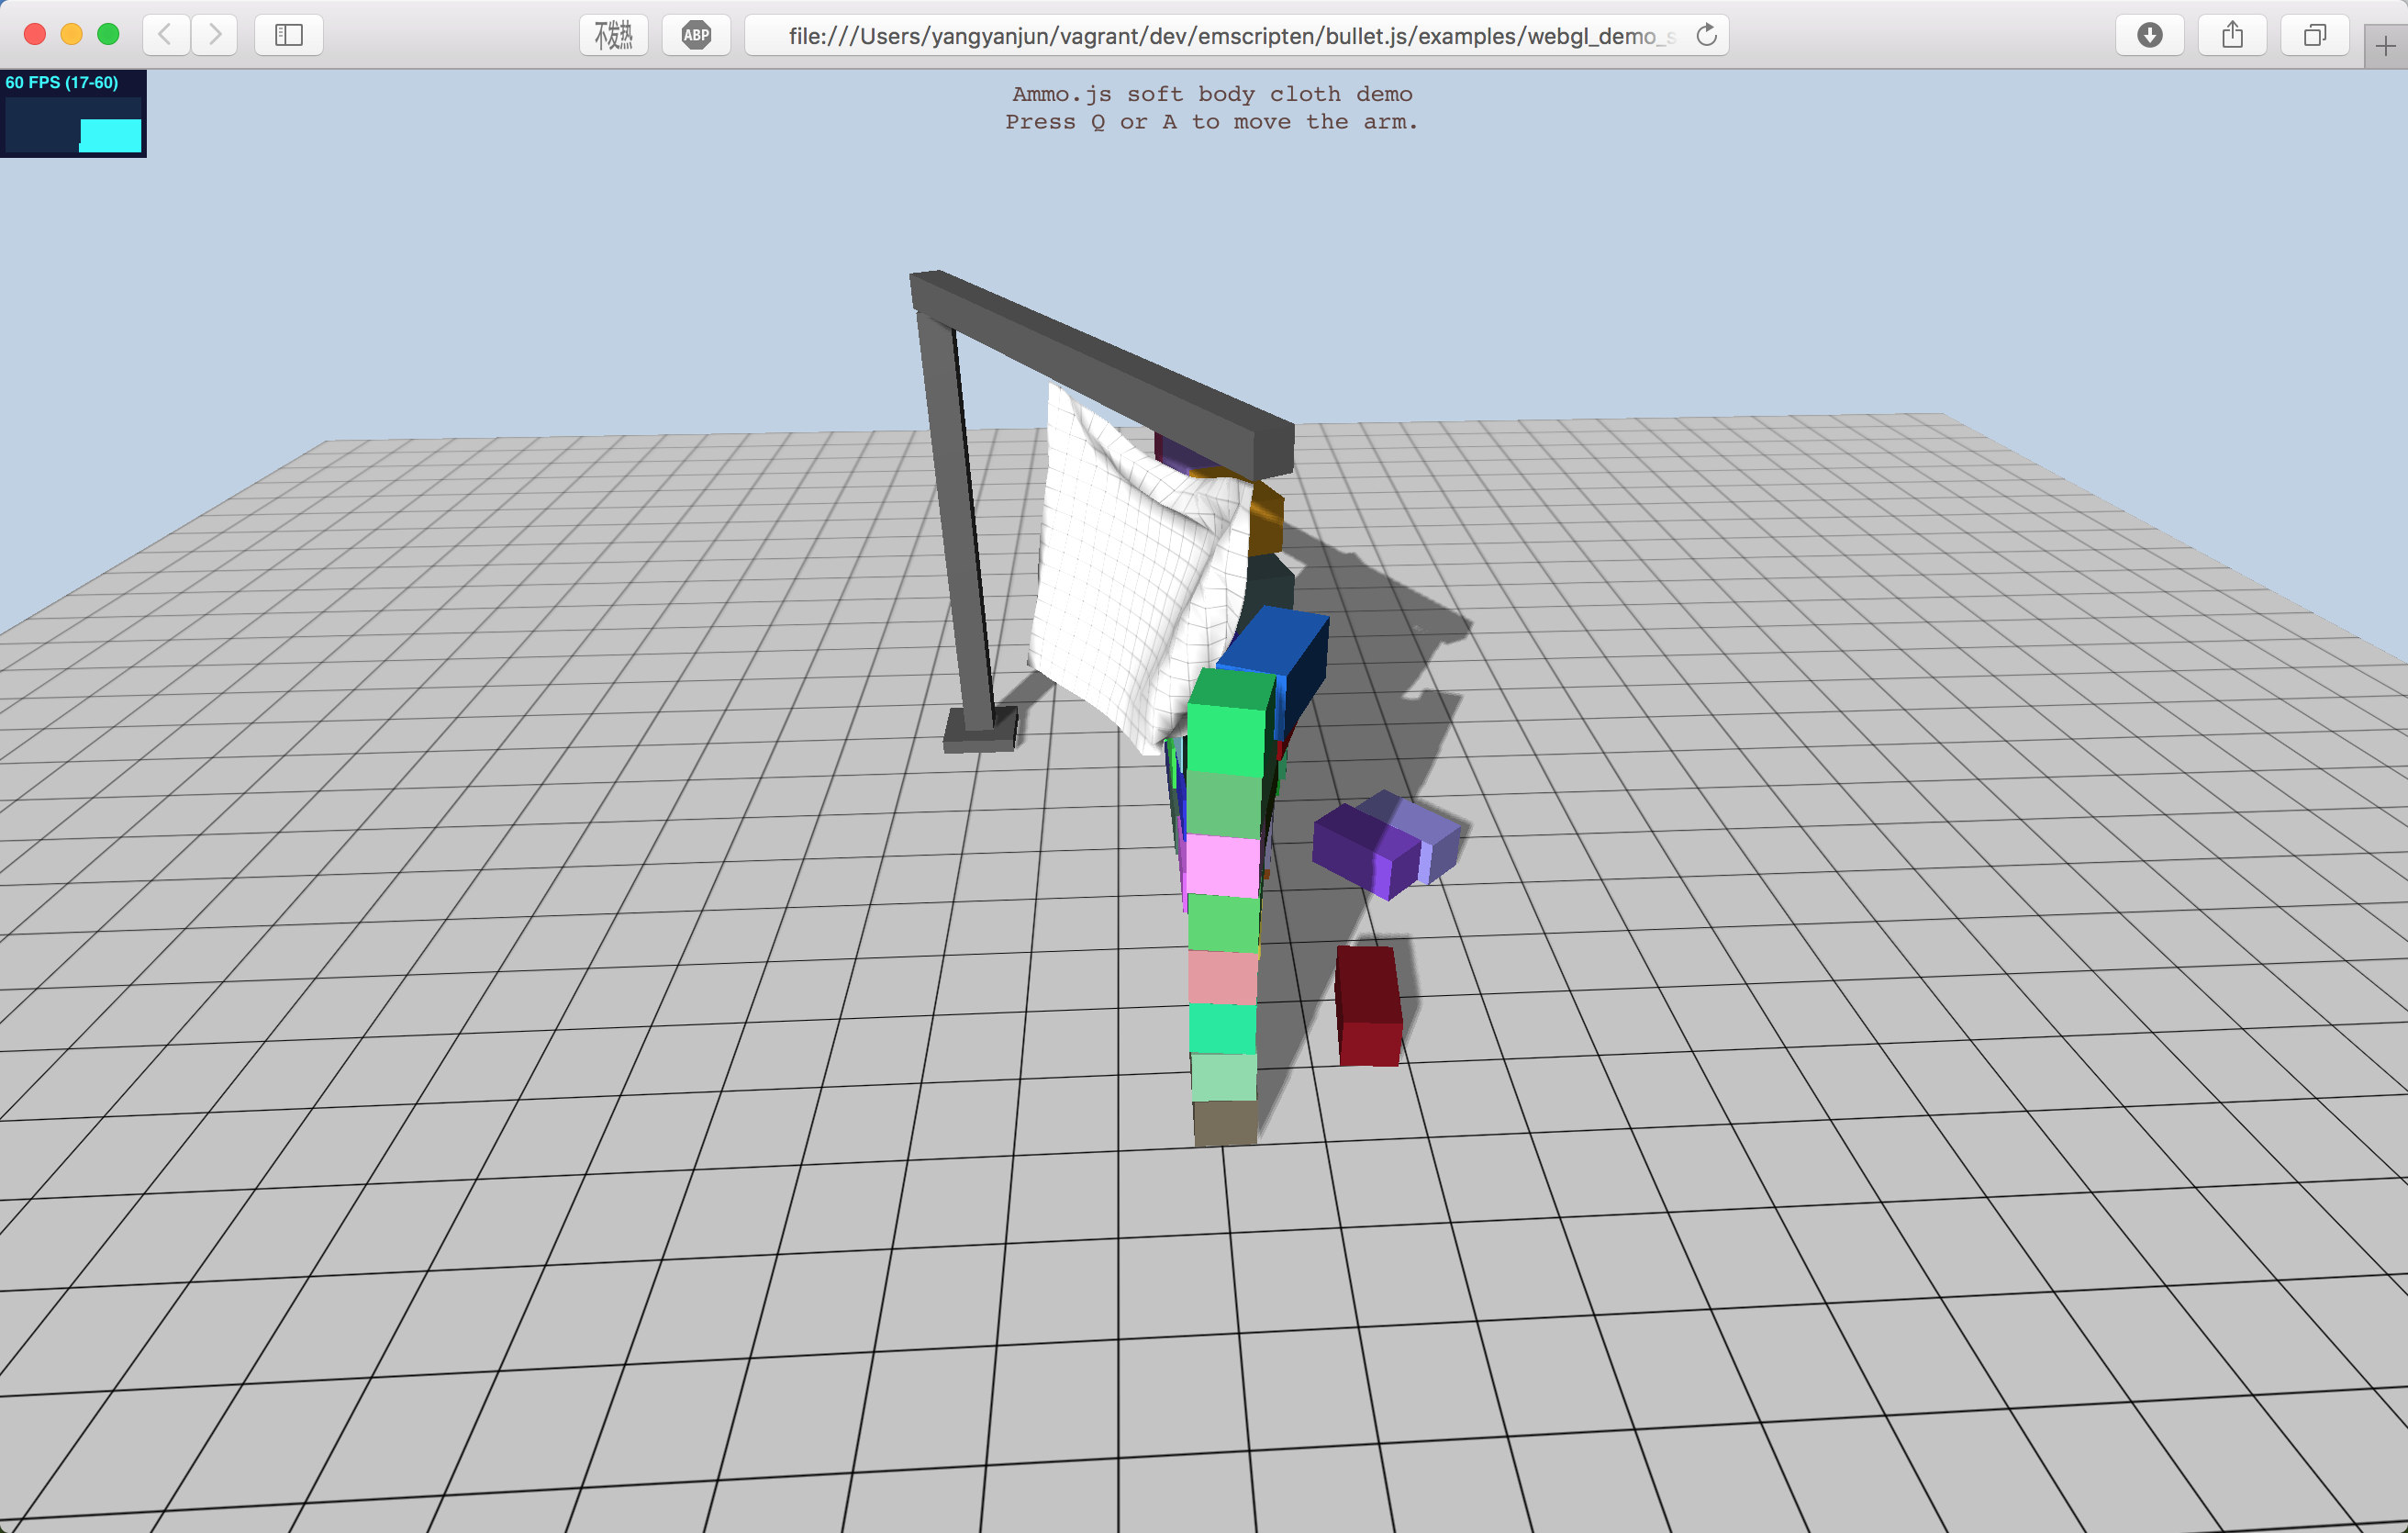
\includegraphics[width=450bp]{figure/pic/ammo-cloth.png}
    \caption{bullet引擎柔体模拟效果}
    \label{ammo-cloth}
\end{figure}

